\documentclass{beamer}
%\usepackage{bookman}
\usetheme{Berkeley}
% choose color scheme
\usecolortheme{dolphin}

\title[Sweave Basics]{ Brief Tour of Sweave Basics}
\author[A. Beale ]{Alan Beale}
\date[May 2011]{May 15, 2011}
\begin{document}
\setbeamercovered{invisible}
\graphicspath{{images//}}

\begin{frame} [plain]
  \titlepage
\end{frame}

\begin{frame}{Why I use Sweave to combine R and Latex}
 \begin{block}<2->
   {Aspirational Programming}
\end{block}

\begin{center}

\includegraphics[scale=.4]{thumb-OprahWinfrey}
\end{center}
\end{frame}

\begin{frame}{Why I use Sweave to combine R and Latex}
 \begin{block}
   {Competing Forces}
\end{block}
\pause
\begin{columns}[t] 
\column{.5 \textwidth}
\begin{center}
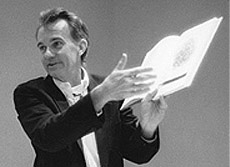
\includegraphics[scale=.4]{etufte}
\end{center}
\pause 
\column{.5 \textwidth}
\begin{center}

\includegraphics[scale=.4]{billgates}
\end{center}
\end{columns}
\end{frame}

\begin{frame}{Why I use Sweave to combine R and Latex}
\begin{block}
   {Literate Programming}
\end{block}
 
\pause
\begin{columns}[t] 
\column{.5 \textwidth}
\begin{center}

\includegraphics[scale=.4]{humor-donald-knuth-jokes-24307359}
\end{center}
\pause 
\column{.5 \textwidth}
\begin{center}
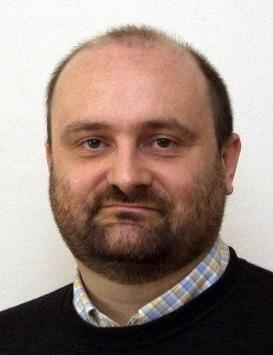
\includegraphics[scale=1.2]{Leisch}
\end{center}
\end{columns}
\end{frame}

\begin{frame} {R Code and results in document}
\end{frame}
\begin{frame} {R code with hidden results?}
\end{frame}

\begin{frame} {R Code producing a figure}
\end{frame}
\begin{frame} {R Code producing a table}
\end{frame}
\begin{frame} {Running Sweave}
\end{frame}

\begin{frame} {Running Stangle}
\end{frame}
\begin{frame} {Benefits and Limitations}
\end{frame}


\end{document}
